\section{Merging $k$ Totally Ordered Sets}
\label{tree:merging:kgeq3}


\subsection*{ITLB}
\label{tree:merging:kgeq3:ITLB}


\begin{theorem}
The \concept{ITLB} for the merging problem when $k \geq 3$ with $|\S_i| = n_i$ and $n =
\sum_{i=1}^{k} n_i$ is \BigOmega{\log \frac{n}{n_1 \cdot n_2 \dots n_k}}.
\end{theorem}

\begin{proof}
We have to choose the $n_1$ positions among $n$ in $\S'$ for the elements of
$\S_1$ and then recursively make this choice on the remaining $n - n_1$
positions with the elements of \(\S_2 \cup \dots \cup \S_k\). The number of
leaves of the decision tree is $\frac{n}{n_1 \cdot n_2 \dots n_k}$ hence the
worst-case minimal height of the tree is $\log \frac{n}{n_1 \cdot n_2 \dots
n_k}$.
\end{proof}

\nb{Giving $\log \frac{n}{n_1 \cdot n_2 \dots n_k}$ in the form of the
Stirling's approximation gives us \(n \log n - \sum_{i=1}^{k} n_i \log n_i -
\BigO{k}\)
which clearly express the information contained in the sorted sequence $\S'$ of
$n$ elements minus the information we already have.}

\subsection*{An Algorithm for the General Merging Problem}
\label{tree:merging:kgeq3:alg}

Our optimal algorithm for the General Merging Problem is as follows.

\begin{algorithm}
\item[1.] Let \(\S_i\) and \(\S_j\) be the two smallest sets from \(\S_1 ,
\dots , \S_k\).
\item[2.] Merge \(\S_i\) and \(\S_j\) with an optimal algorithm.
\item[3.] Merge \((\enum{\S_1 , \dots , \S_k} \setminus \enum{\S_i,\S_j} )
\cup \enum{\S_i \cup \S_j}\).
\end{algorithm}

We will use tools of Information Theory to prove that this algorithm is
optimal. The first tool we will be using is Shannon's entropy, \(H(X)\).
\begin{theorem}
\begin{displaymath}
H(X) = \sum_{x_i} p(x_i) \log \frac{1}{p(x_i)}.
\end{displaymath}
\end{theorem}

Let us take some time to expose the relation between constructions of Huffman
codes and runs of our algorithm. First, we define the problem of optimal
coding of a random variable with respect to the average length of the messages
encoding events emitted by this random variable. We assume the channel we
use to transmit our messages is perfect:

\begin{problem}
Given a random variable \(X\) with possible event \(x_1,\ldots,x_n\) occuring
with probability \(0 < p(x_i) \le 1, \sum_{x_i} p(x_i) = 1\), construct an
instantaneous code to transmit events through a perfect channel with alphabet
\(\Sigma = \enum{0,1}\) that minimizes the average size of a message encoding
an event.
\end{problem}

The are several results on this subject which we summarize in the
following theorem,

\begin{theorem}
The average code length \(L(X)\) of any instantaneous coding scheme can not be smaller than
the entropy of the random variable \(H(X)\). If we define by \(l(x_i)\) to be the code
length for event \(x_i\), then the average code length is
\begin{displaymath}
L(X) = \sum_{x_i} p(x_i) l(x_i).
\end{displaymath}
With respect to the objective function we mentioned above, Huffman coding is
an optimal instantaneous code and its average length \(L_H(X)\) is bounded by
\begin{displaymath}
H(X) \le L_H(X) \le H(X) + 1.
\end{displaymath}
\end{theorem}

\(L_H(X)\) is achieved by constructing a Huffman tree. The method to build this
tree is the following. We start with \(n\) leaves, one for each possible event
\(x_i\). We assign a weight of \(p(x_i)\) to each of these leaves. The current
structure is not quite a tree but a pool of disconnected nodes.  Then, one
replaces the two nodes of the pool with smallest weight by a new one which will
act as their parent in the Huffman tree. The weight of this new node is
computed as the sum of the weights of its children. One repeats this
replacement operation until the pool contains only one element. This last
element is the root of the tree. Since at each step we replace two nodes by
one, after \(n-1\) of these steps the tree is constructed.

Now we make the parallel with our merging algorithm. If we want to merge
multiple totally ordered sets \(\S_1,\ldots,\S_k\) having different lengths we can use a similar
approach. To each set \(\S_i\) we assign a fake event with probability
\(\frac{\card{\S_i}}{n}\) hence the Shannon entropy of the random variable
\(S\) with this probability distribution is
\begin{align}
H(S) &= - \sum \frac{\card{\S_i}}{n} \log \frac{\card{\S_i}}{n}\\
&= - \sum \frac{\card{\S_i}}{n} (\log \card{\S_i} - \log n)\\
&= \sum \frac{\card{\S_i}}{n} \log n - \sum \frac{\card{\S_i}}{n} \log \card{\S_i}\\
&= \frac{1}{n} \sum \card{\S_i} \log n - \frac{1}{n} \sum \card{\S_i} \log
\card{\S_i}\\
&= \frac{1}{n} (n \log n - \sum \card{\S_i} \log \card{\S_i})\\
\end{align}

The definition of \(p(\S_i)\) is consistent with the invariant of
the Huffman tree construction algorithm since merging two totally ordered sets
\(\S_i\) and \(\S_j\) produces a new one of size \(\card{\S_i} + \card{\S_j}\).

Now we prove that for a merging algorithm that would iteratively merge the two
smallest remaining totally ordered set, the number of comparison used is at
most \(n L_H(\S)\). To make this explicit, we rearrange the terms of \(L(\S_i)\),

\begin{displaymath}
L_H(\S) = \sum \frac{\card{\S_i}}{n} l(\S_i) = \frac{1}{n} \sum l(\S_i) \card{\S_i}.
\end{displaymath}

In the above equation, \(l(\S_i)\) corresponds to the number of times elements
of \(\S_i\) are taking part in a merge operation. When merging two totally
ordered sets \(\S_i\) and \(\S_j\) the standard Tapemerge algorithm uses less
than \(\card{\S_i} + \card{\S_j}\) comparisons. Moreover, the totally ordered set
associated to a node of the Huffman tree is the union of the totally ordered
sets associated to \(u\) leaves of the tree. These leaves are
\(\S_{i_1},\ldots,\S_{i_u}\) and have lengths
\(\card{\S_{i_1}},\ldots,\card{\S_{i_u}}\). When two nodes are merged, it
requires thus less than
\(\card{\S_{i_1}}+\ldots+\card{\S_{i_u}}+\card{\S_{j_1}}+\ldots+\card{\S_{j_v}}\)
comparisons. We can rearrange these \(\card{\S_{i_w}}\) and conclude that
\(\sum l(\S_i) \card{\S_i}\) is an upper bound on the number of comparisons used
by our algorithm. Since,
\begin{displaymath}
n H(\S) \le n L_H(\S) \le n H(\S) + n,
\end{displaymath}
our algorithm requires at most \(n \log n - \sum \card{\S_i} \log \card{\S_i} +
n\) comparisons which is \(\concept{ITLB} + \BigO{n}\).

To handle sublinear \concept{ITLB} we need
to resort to a last trick. The only way the \concept{ITLB} can be \SmallO{n}
is if the last two nodes \(\U\) and \(\L\) we merge have sizes \(m\) and \(n\)
respectively such that \(m =
\SmallO{n}\). Otherwise merging them would require \BigOmega{n} comparisons.
If \(m = \SmallO{n}\), then we can use the Hwang-lin algorithm to merge those
two nodes optimally in \BigO{m \log \frac{n}{m}} comparisons. Moreover, the
set \(\L\) can only be a leaf of the Huffman tree. Indeed, it can
not be the result of a merge operation between two \BigO{m} sized nodes.
Since this is the only kind of merge operation that is allowed before having
merged the set \(\U\) with another one, \(\L\) is necessarily a leaf.
Producing the totally ordered set of size \(m\) uses at most \BigO{m \log m}
comparisons. Since \(\BigO{m \log m} = \BigO{m \log \frac{n}{m}}\) when \(m =
\SmallO{n}\), after trading the Tapemerge algorithm for the Hwang-Lin
algorithm our algorithm is optimal.

Our algorithm is thus building the Huffman tree and then merges the two deepest
leaves of the Huffman tree using the Hwang-Lin algorithm until there is only
one leaf left.

\begin{figure}
	\centering
	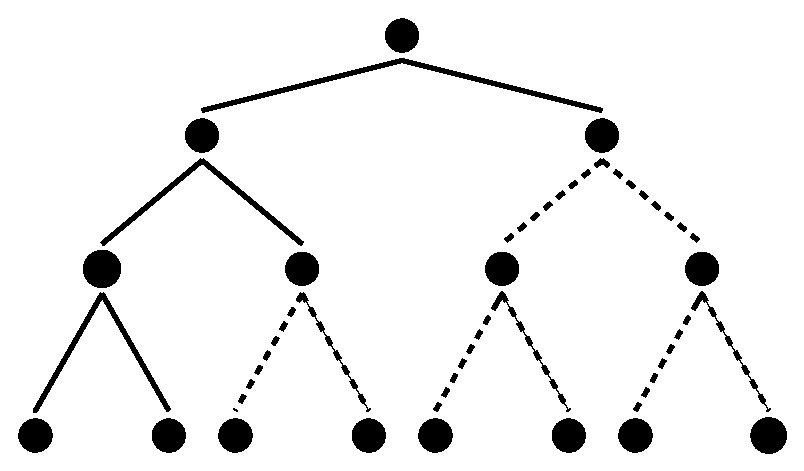
\includegraphics[width=0.4\textwidth]{fig/merging/huffman-2-trim}
	\caption{Complexity of the merging problem as a difference between the whole merge process and its subprocesses.}
	\label{tree:merging:fig/huffman-2}
\end{figure}

We provide a visual way of understanding these results. Looking at
\ref{tree:merging:fig/huffman-2} we can deduce the complexity of the algorithm.
The dashed lines in \ref{tree:merging:fig/huffman-2} represent steps producing
information we already have. Since those steps do not need to be processed, and
since they normally would have required us to make \(\BigO{n \log n}\) queries, we have a
total complexity of $\BigO{n \log n - \sum_{i=1}^{k} n_i \log n_i} =
\BigO{ITLB}$ where $n_i$ is the cardinality of the $i$-th totally ordered set
of the input.
